
\chapter{Resultados\label{chap:Resultados}}

% Resumo opcional. Comentar se não usar.
%\resumodocapitulo{resumo opcional}

%\section{Resultados}

\section{Teste preliminar} \label{sect:testepreliminar}

Durante testes preliminares, o analisou-se a variação dos valores de RSSI e frequência Doppler com uma única TAG e uma única antena. A princípio as leituras pareciam muito sujeitas a ruído e pequenas alterações, então foram aplicados dois filtros: um filtro passa altas com corte em -60dB para o sinal de RSSI e um filtro rejeita banda para frequência Doppler para ignorar leituras menores que -1,50Hz e maiores que 1,50Hz. O teste preliminar resultou na figura \ref{fig:teste_preliminar}.
 
 \begin{figure}[ht]
    \centering
    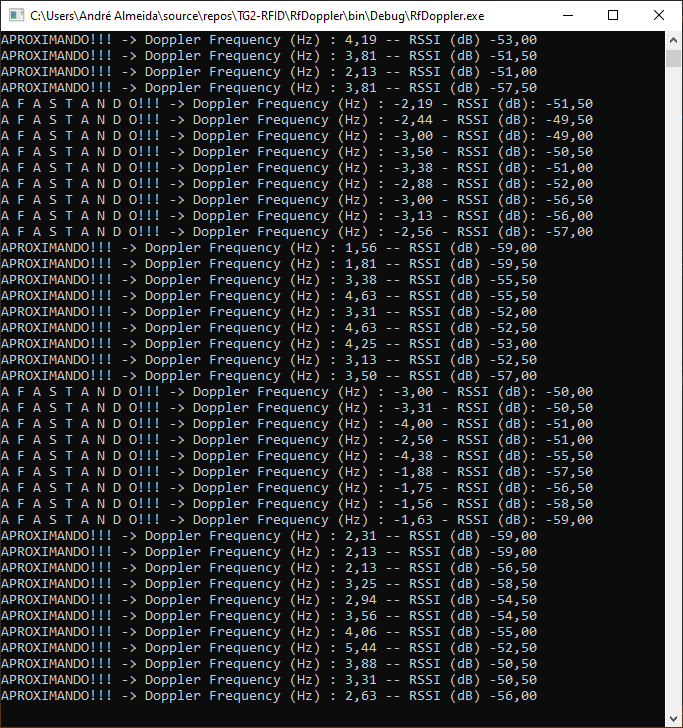
\includegraphics[width=0.7\linewidth]{figs/Metodologia/teste_doppler+RSSI_corte_60db.PNG}
    \caption{Captura de tela mostrando os dados de frequência Doppler e potência RSSI capturados no teste preliminar}
    \label{fig:teste_preliminar}
\end{figure}
 
 O teste se mostrou bastante promissor, pois é possível observar na figura \ref{fig:teste_preliminar} que realizando as configurações corretas e aplicando filtros para rejeitar \textit{outliers} de leitura é possível extrair informações úteis das leituras. Neste teste o valor da frequência Doppler foi observado para definir se a TAG se aproxima ou se afasta da antena.
 
 Ainda é possível perceber que as leituras de frequência Doppler e RSSI, seguem tendências bem definidas. As leituras de frequência Doppler são positivas ao aproximar a TAG da antena, e negativas ao afastar a TAG da antena. A transição entre leituras positivas e negativas ocorre no exato momento de passagem na frente da leitora. As leituras de potência RSSI tentem a ser maiores no momento em que a pessoa está mais próxima da antena, e menores a medida em que se afasta da antena.
 
 Apesar de seguirem uma tendência bem definida, possuem variações abruptas, algumas vezes no sentido oposto ao esperado. Por exemplo, observa-se uma queda abrupta de -51,00 dB e -52,50 dB para -57,00 dB nas duas transições entre o momento em que a pessoa se aproxima e o momento em que a pessoa se afasta da antena. Quanto ao efeito Doppler, este é proporcional à velocidade da pessoa, entretanto, o caminhar de uma pessoa não segue uma velocidade constante a todo momento, e portanto nota-se uma flutuação constante no valor lido.

\section{Teste do programa implementado}

O \textit{software} criado para este trabalho segue a metodologia e as estratégias mencionadas na sessão \ref{section:estrategias}. O programa foi construído de tal forma que, ao mesmo tempo, é possível realizar todos os seis casos de teste. Para isso, a classe \textit{cardholder} possui sete variáveis para armazenar ambientes: uma para o ambiente real - indicado manualmente no terminal do programa quando executado em modo \textit{debug}, para uma pessoa específica apenas - e seis para as suposições de ambiente atual de cada caso de teste.

Três testes foram executados e, durante a execução, o programa armazenou, em tempo real, os dados relevantes de cada leitura de TAG (nome do portador da TAG, número EPC, nome da leitora, número da antena que capturou a leitura, data, horário da captura das informações, ambiente atual, curva de valores de potência RSSI, curva de frequência Doppler e as seis hipóteses de ambiente atual geradas pelos casos de teste). Estes dados podem ser vistos nos apêndices \ref{apendix:1}, \ref{apendix:2} e \ref{apendix:3}.

Durante a execução do primeiro teste, uma pessoa transitou pelo ambiente do LARA, enquanto outra registrava manualmente os valores de ambiente real (apêndice \ref{apendix:1}). Durante a execução dos dois testes seguintes (apêndices \ref{apendix:2} e \ref{apendix:3}), uma pessoa percorreu o LARA enquanto outra filmou o percurso para validação dos dados, comparando os tempos no vídeo e os registros de \textit{log} do programa.

Durante a execução do primeiro e do terceiro testes (apêndices \ref{apendix:1} e \ref{apendix:3}) caminhou-se a velocidade constante em frente às leitoras. O segundo teste (apêndice \ref{apendix:2}) envolveu mudanças bruscas de direção no momento do cruzamento das fronteiras.

As figuras \ref{fig:cruzamento01}, \ref{fig:cruzamento10}, \ref{fig:cruzamento12}, \ref{fig:cruzamento21}, \ref{fig:cruzamento13} e \ref{fig:cruzamento31} mostram imagens dos vídeos gravados, durante os cruzamentos de fronteira entre ambientes, em frente às leitoras e às antenas.


\begin{figure}[H]
    \centering
    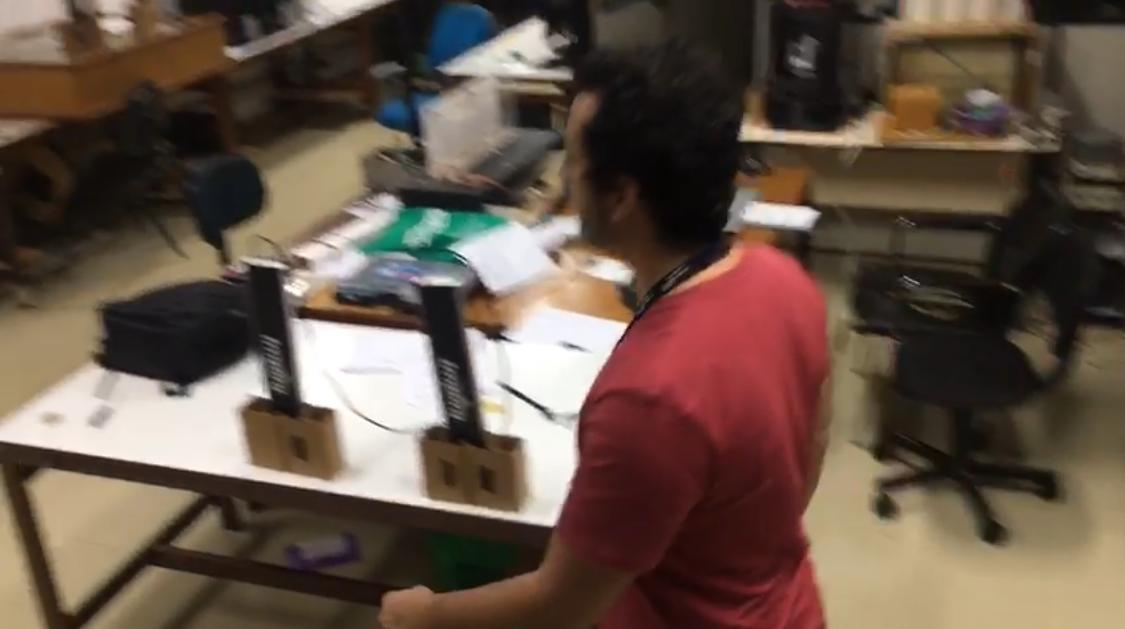
\includegraphics[width=0.5\linewidth]{figs/Resultados/cruzamento01.jpeg}
    \caption{Teste do programa - Leitura do cruzamento da fronteira de Área Externa (0) para Sala Principal (1)}
    \label{fig:cruzamento01}
\end{figure}

\begin{figure}[H]
    \centering
    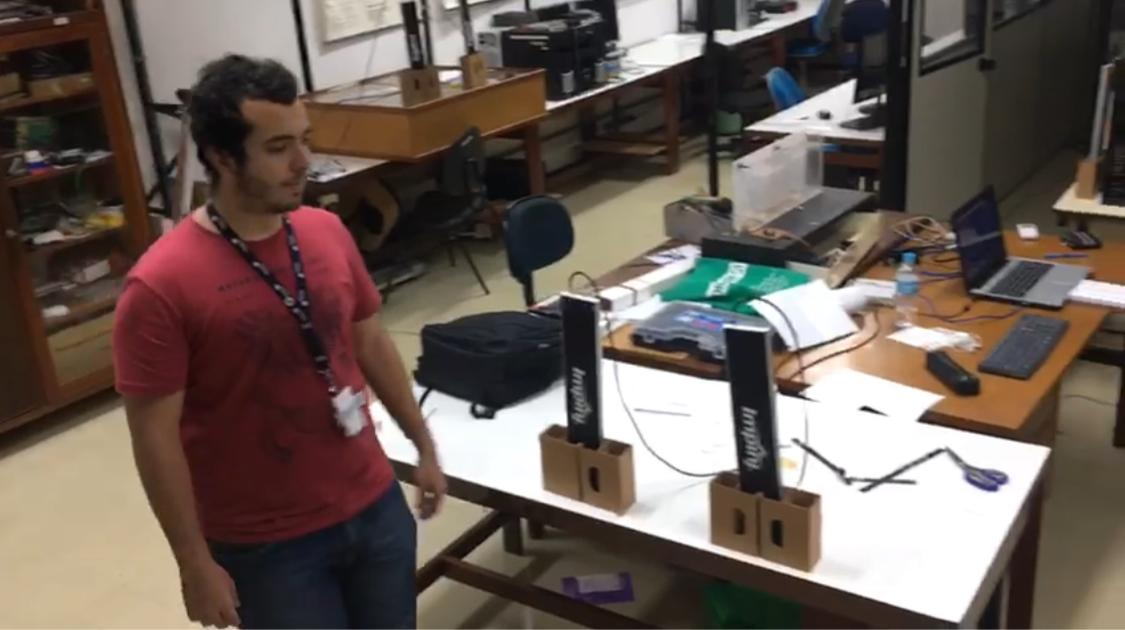
\includegraphics[width=0.5\linewidth]{figs/Resultados/cruzamento10.jpeg}
    \caption{Teste do programa - Leitura do cruzamento da fronteira de Sala Principal (1) para Área Externa (0)}
    \label{fig:cruzamento10}
\end{figure}

\begin{figure}[H]
    \centering
    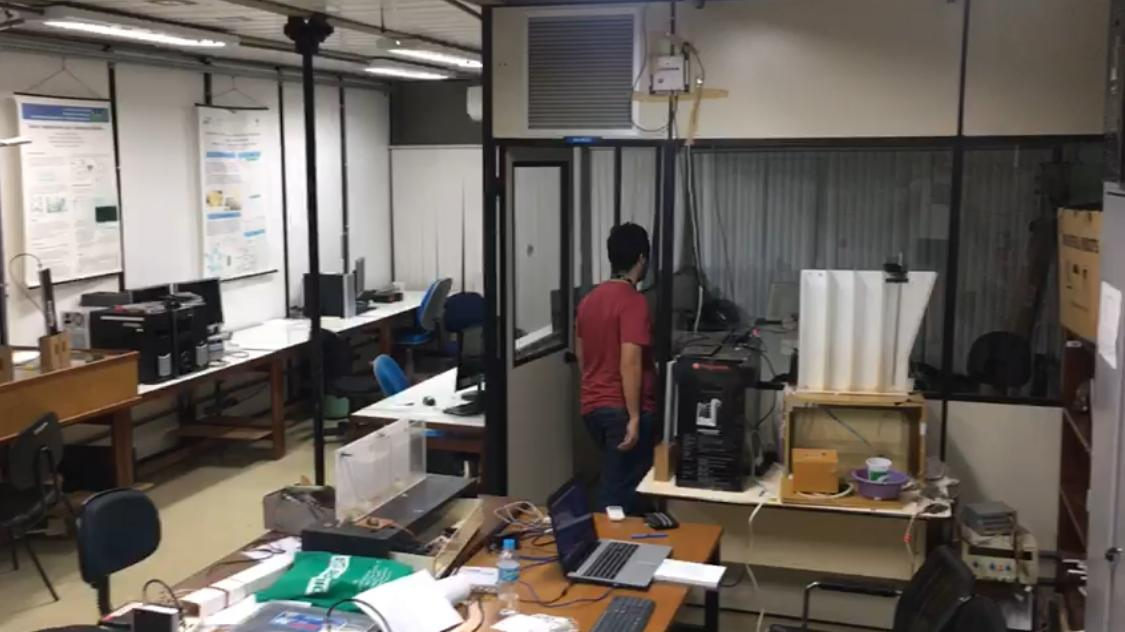
\includegraphics[width=0.5\linewidth]{figs/Resultados/cruzamento12.jpeg}
    \caption{Teste do programa - Leitura do cruzamento da fronteira de Sala Principal (1) para Sala de Reuniões (2)}
    \label{fig:cruzamento12}
\end{figure}

\begin{figure}[H]
    \centering
    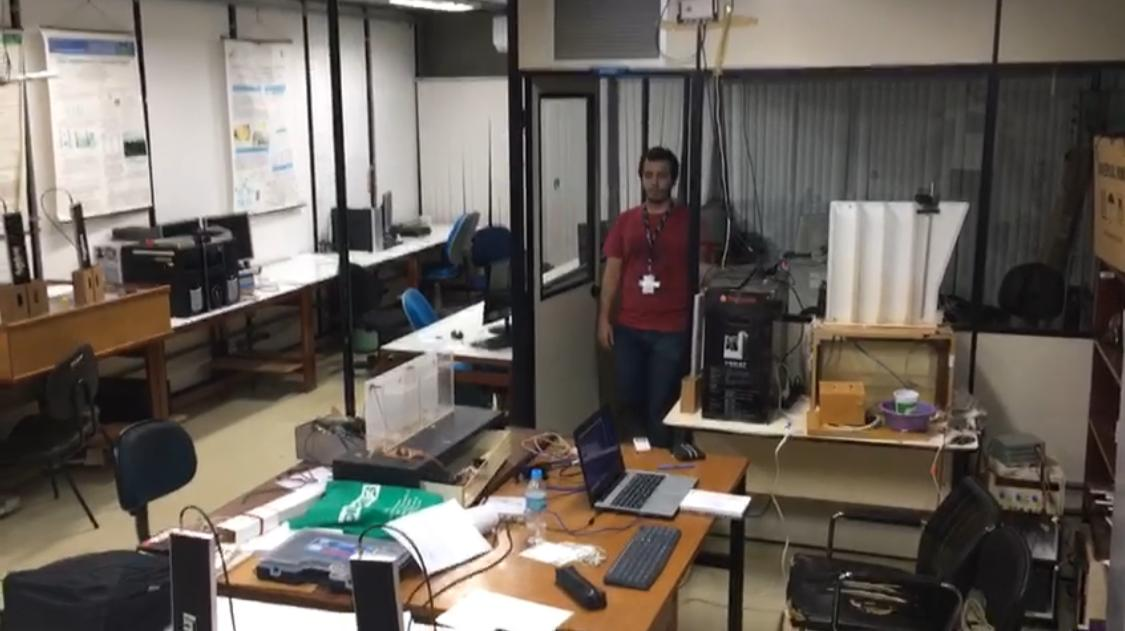
\includegraphics[width=0.5\linewidth]{figs/Resultados/cruzamento21.jpeg}
    \caption{Teste do programa - Leitura do cruzamento da fronteira de Sala de Reuniões (2) para Sala Principal (1)}
    \label{fig:cruzamento21}
\end{figure}

\begin{figure}[H]
    \centering
    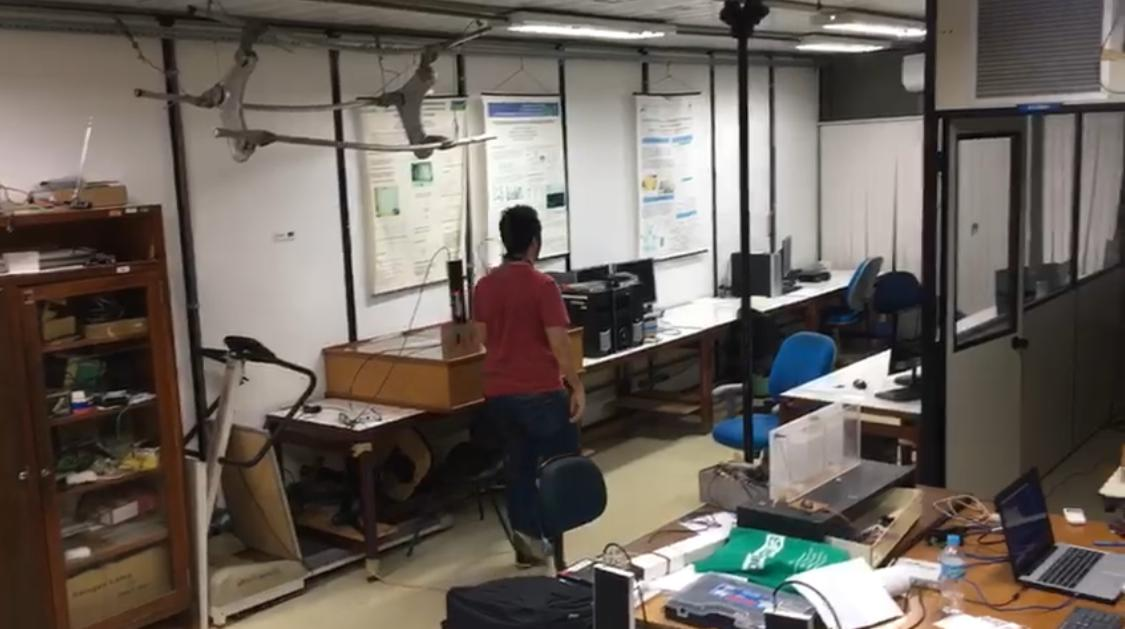
\includegraphics[width=0.5\linewidth]{figs/Resultados/cruzamento13.jpeg}
    \caption{Teste do programa - Leitura do cruzamento da fronteira de Sala Principal (1) para Corredor Baias(3)}
    \label{fig:cruzamento13}
\end{figure}

\begin{figure}[H]
    \centering
    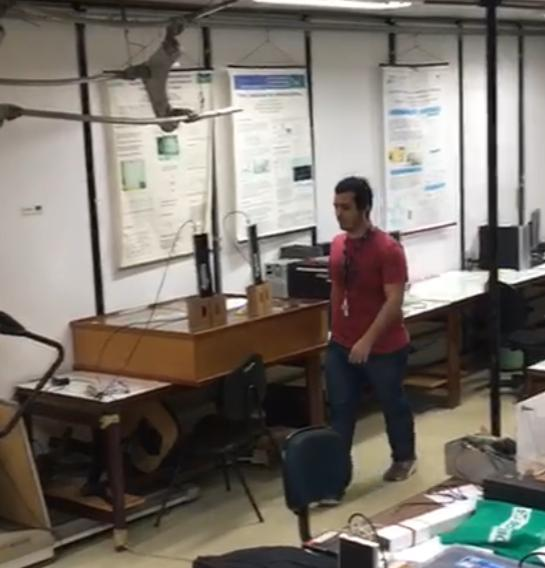
\includegraphics[width=0.5\linewidth]{figs/Resultados/cruzamento31.jpeg}
    \caption{Teste do programa - Leitura do cruzamento da fronteira de Corredor Baias(3) para Sala Principal (1)}
    \label{fig:cruzamento31}
\end{figure}

\section{Eficiência dos critérios}

\subsection{Comparação do último valor de RSSI} \label{section:ultimovalorRES}

A eficiência do critério de último valor de RSSI baseada no caso de teste do apêndice \ref{apendix:1} pode ser vista na tabela \ref{tab:resultados1}

\begin{table}[H]
\centering
\caption{Eficiência do critério do último valor com base no teste do apêndice \ref{apendix:1} }
\label{tab:resultados1}
\begin{tabular}{p{5cm} p{5cm}}
\hline
\multicolumn{2}{c}{\cellcolor{lightgray}{Eficiência do critério: Último valor de RSSI}} \\ \hline
Leituras certas         &   $102 / 129$        \\
Confiabilidade crua    &   $79\%$     \\
Erros confirmados          &  $2 /10$        \\
Confiabilidade analítica & $80\%$ \\ \hline
\end{tabular}
\end{table}

As leituras certas são uma comparação exata com o valor indicado em "ambiente atual", de entrada do usuário. A confiabilidade crua divide a quantidade de erros identificados pela quantidade total de leituras, que neste caso foram 129, e mostra a confiabilidade do método. Os erros confirmados foram digitados manualmente, analisando-se todo o percurso e identificando que muitas das leituras erradas foram corrigidas pelo programa logo após, pois as curvas precisam de algumas leituras a mais para processar os casos de teste e por isso foram contabilizados apenas os erros não corrigidos após diversas leituras. A confiabilidade analítica divide a quantidade de erros contabilizados manualmente pela quantidade de transições de ambiente efetuadas, que, neste caso, foram 10 transições.


\subsection{Comparação dos tempos dos últimos picos de RSSI}

A eficiência do critério dos tempos de pico de RSSI baseada no caso de teste do apêndice \ref{apendix:1} pode ser vista na tabela \ref{tab:resultados2}

\begin{table}[H]
\centering
\caption{Eficiência do critério dos tempos de picos de RSSI com base no teste do apêndice \ref{apendix:1} }
\label{tab:resultados2}
\begin{tabular}{p{5cm} p{5cm}}
\hline
\multicolumn{2}{c}{\cellcolor{lightgray}{Eficiência do critério: Tempos de pico de RSSI}} \\ \hline
Leituras certas         &   $102 / 129$        \\
Confiabilidade crua    &   $79\%$     \\
Erros confirmados          &  $2 / 10$        \\
Confiabilidade analítica & $80\%$ \\ \hline
\end{tabular}
\end{table}

Os itens de erro e confiabilidade desta tabela são os mesmos do caso de teste de último valor, sessão \ref{section:ultimovalorRES}, já que foram executados no mesmo teste. Foram 129 leituras e 10 transições de ambiente.


\subsection{Comparação da média dos valores de RSSI}

A eficiência do critério média dos valores de RSSI baseada no caso de teste do apêndice \ref{apendix:1} pode ser vista na tabela \ref{tab:resultados3}

\begin{table}[H]
\centering
\caption{Eficiência do critério da média dos valores de RSSI com base no teste do apêndice \ref{apendix:1} }
\label{tab:resultados3}
\begin{tabular}{p{5cm} p{5cm}}
\hline
\multicolumn{2}{c}{\cellcolor{lightgray}{Eficiência do critério: Média dos valores de RSSI}} \\ \hline
Leituras certas         &   $40 / 129$        \\
Confiabilidade crua    &   $31\%$     \\
Erros confirmados          &  $9 / 10$        \\
Confiabilidade analítica & $10\%$ \\ \hline
\end{tabular}
\end{table}

Os itens de erro e confiabilidade desta tabela são os mesmos do caso de teste de último valor, sessão \ref{section:ultimovalorRES}, já que foram executados no mesmo teste. Foram 129 leituras e 10 transições de ambiente.

\subsection{Comparação da mediana dos sinais RSSI}

A eficiência do critério mediana dos valores de RSSI baseada no caso de teste do apêndice \ref{apendix:1} pode ser vista na tabela \ref{tab:resultados4}

\begin{table}[H]
\centering
\caption{Eficiência do critério da mediana dos valores de RSSI com base no teste do apêndice \ref{apendix:1} }
\label{tab:resultados4}
\begin{tabular}{p{5cm} p{5cm}}
\hline
\multicolumn{2}{c}{\cellcolor{lightgray}{Eficiência do critério: Mediana dos valores de RSSI}} \\ \hline
Leituras certas         &   $41 / 129$        \\
Confiabilidade crua    &   $32\%$     \\
Erros confirmados          &  $4 / 10$        \\
Confiabilidade analítica & $60\%$ \\ \hline
\end{tabular}
\end{table}

Os itens de erro e confiabilidade desta tabela são os mesmos do caso de teste de último valor, sessão \ref{section:ultimovalorRES}, já que foram executados no mesmo teste. Foram 129 leituras e 10 transições de ambiente.

\subsection{Comparação da travessia por Efeito Doppler}


A eficiência do critério de travessia por Efeito Doppler baseada no caso de teste do apêndice \ref{apendix:1} pode ser vista na tabela \ref{tab:resultados5}

\begin{table}[H]
\centering
\caption{Eficiência do critério de travessia por Efeito Doppler com base no teste do apêndice \ref{apendix:5} }
\label{tab:resultados5}
\begin{tabular}{p{5cm} p{5cm}}
\hline
\multicolumn{2}{c}{\cellcolor{lightgray}{Eficiência do critério: Travessia por efeito Doppler}} \\ \hline
Leituras certas         &   $69 / 129$        \\
Confiabilidade crua    &   $53\%$     \\
Erros confirmados          &  $4 / 10$        \\
Confiabilidade analítica & $60\%$ \\ \hline
\end{tabular}
\end{table}

Os itens de erro e confiabilidade desta tabela são os mesmos do caso de teste de último valor, sessão \ref{section:ultimovalorRES}, já que foram executados no mesmo teste. Foram 129 leituras e 10 transições de ambiente.

\subsection{Combinação da técnica de picos de RSSI com Efeito Doppler}

A eficiência do critério de travessia por Efeito Doppler baseada no caso de teste do apêndice \ref{apendix:1} pode ser vista na tabela \ref{tab:resultados6}

\begin{table}[H]
\centering
\caption{Eficiência do critério de combinação de comparação de picos de valores de RSSI e travessia por Efeito Doppler com base no teste do apêndice \ref{apendix:1} }
\label{tab:resultados6}
\begin{tabular}{p{5cm} p{5cm}}
\hline
\multicolumn{2}{c}{\cellcolor{lightgray}{Eficiência do critério: Travessia por efeito Doppler}} \\ \hline
Leituras certas         &   $70 / 129$        \\
Confiabilidade crua    &   $54\%$     \\
Erros confirmados          &  $5 / 10$        \\
Confiabilidade analítica & $50\%$ \\ \hline
\end{tabular}
\end{table}

Os itens de erro e confiabilidade desta tabela são os mesmos do caso de teste de último valor, sessão \ref{section:ultimovalorRES}, já que foram executados no mesmo teste. Foram 129 leituras e 10 transições de ambiente.